\newpage

\paragraph{\LARGE Aufgabe 8 - Dateisysteme}

\section{Aufgabenstellung}
	\begin{quote}
		Impemetieren Sie ein C-Programm, das folgende Anforderungen erf\"ullt:\\ \\
		\begin{enumerate}
			\item Eine Datei wird zum Lesen ge\"offnet; anschließend wird zuerst die zweite H\"alfte und dann die erste H\"alfte des Dateiinhaltes auf dem Bildschirm ausgegeben.\\
			\item Danach wird der Inhalt der Datei in eine neue Datei kopiert, wobei der Dateiname der Quell- und der Zieldatei dem Programm als Argument \"ubergeben werden kann.\\
			\item Die letzten 10 Zeichen der urspr\"unglichen Datei werden ab der 11. Stelle der neuen Datei kopiert. Das Dateiende der neuen Datei soll jetzt nach den verschobenen Daten sein (also nach dem 21. Zeichen).\\
			\item Der Inhalt der Datei soll auf dem Bildschirm ausgegeben werden.\\
		\end{enumerate}
		Hinweise:\\ \\
		\begin{enumerate}
			\item Benutzen Sie f\"ur diese Aufgabe ausschließlich die POSIX Befehle zur Dateibehandlung und zur Bildschirmausgabe.\\
			\item Die in Frage kommenden POSIX Befehle sind z.B.: open, close, lseek, read, write, ftruncate\\
			\item Die Standard C-Bibliotheksfunktionen wie z.B. fopen, fprintf, printf usw. d\"urfen in Ihren Programm ausschließlich zu Debugzwecken benutzt werden.\\
			\item Bildschirmausgabe und Kopieren einer Datei sollen in derselben Funktion realisiert werden. Das Ziel der Operation (Standardausgabe oder Zieldatei) wird der Funktion als Parameter \"ubergeben.\\
			\item Es sollen keinerlei Beschr\"ankungen \"uber die Gr\"oße der zu kopierenden Inhalte getroffen werden.\\
			\item Fehlerausgaben (z.B. eine Datei kann nicht ge\"offnet werden) sollen auf stderr erfolgen.\\
			\item Eine Dokumention der ben\"otigten POSIX Aufrufe finden Sie z.B. hier:\\
			http://www.opengroup.org/onlinepubs/009695399/functions/contents.html\\
		\end{enumerate}
	\end{quote}
\newpage
\section{Aufgabe 8.1}
	\subsection{Vorbereitung}
		\begin{quote}
			C-Projekt anlegen.\\
			Makefile schreiben.\\
		\end{quote}
	\subsection{Durchführung}
		\begin{quote}
			Code schreiben und dann testen bzw debuggen.\\
		\end{quote}
	\subsection{Fazit}
		\begin{quote}
			Aufgabe 8.1.1:\\ \\
			\small\lstinputlisting[language=C, firstline=88, lastline=120]{../src/mycp.c}
			\normalsize Zuerst wird mit ''open(quelldatei, O\_RDONLY)'' die Quelldatei ge\"offnet. Dann wird die Position des letzten Zeichens/Bytes mit ''lseek(datei, -1L, SEEK\_END)'' ermittelt. Dieser Wert wird dann durch Zwei geteilt dann hat man die Dateimitte. Danach wird die Lese/Schreib-Markierung mit ''lseek(datei, dateiMitte, SEEK\_SET)'' zur Dateimitte verschoben. Dann wird die Datei blockweise mit ''read()'' eingelesen und mit ''write(1, buffer, count);'' auf dem Bildschirm ausgegeben bis das Dateiende erreicht ist. Danach wird die Lese/Schreib-Markierung mit ''lseek(datei, 0L, SEEK\_SET);'' wieder zum Anfang verschoben. Danach wird die Datei wieder blockweise mit ''read()'' eingelesen und mit ''write(1, buffer, count);'' auf dem Bildschirm ausgegeben solange die Lese/Schreib-Markierung kleiner als die Dateimitte ist. Die Position der Lese/Schreib-Markierung  wird mit ''pos += count;'' bei jeden Durchgang ermittelt.\\
			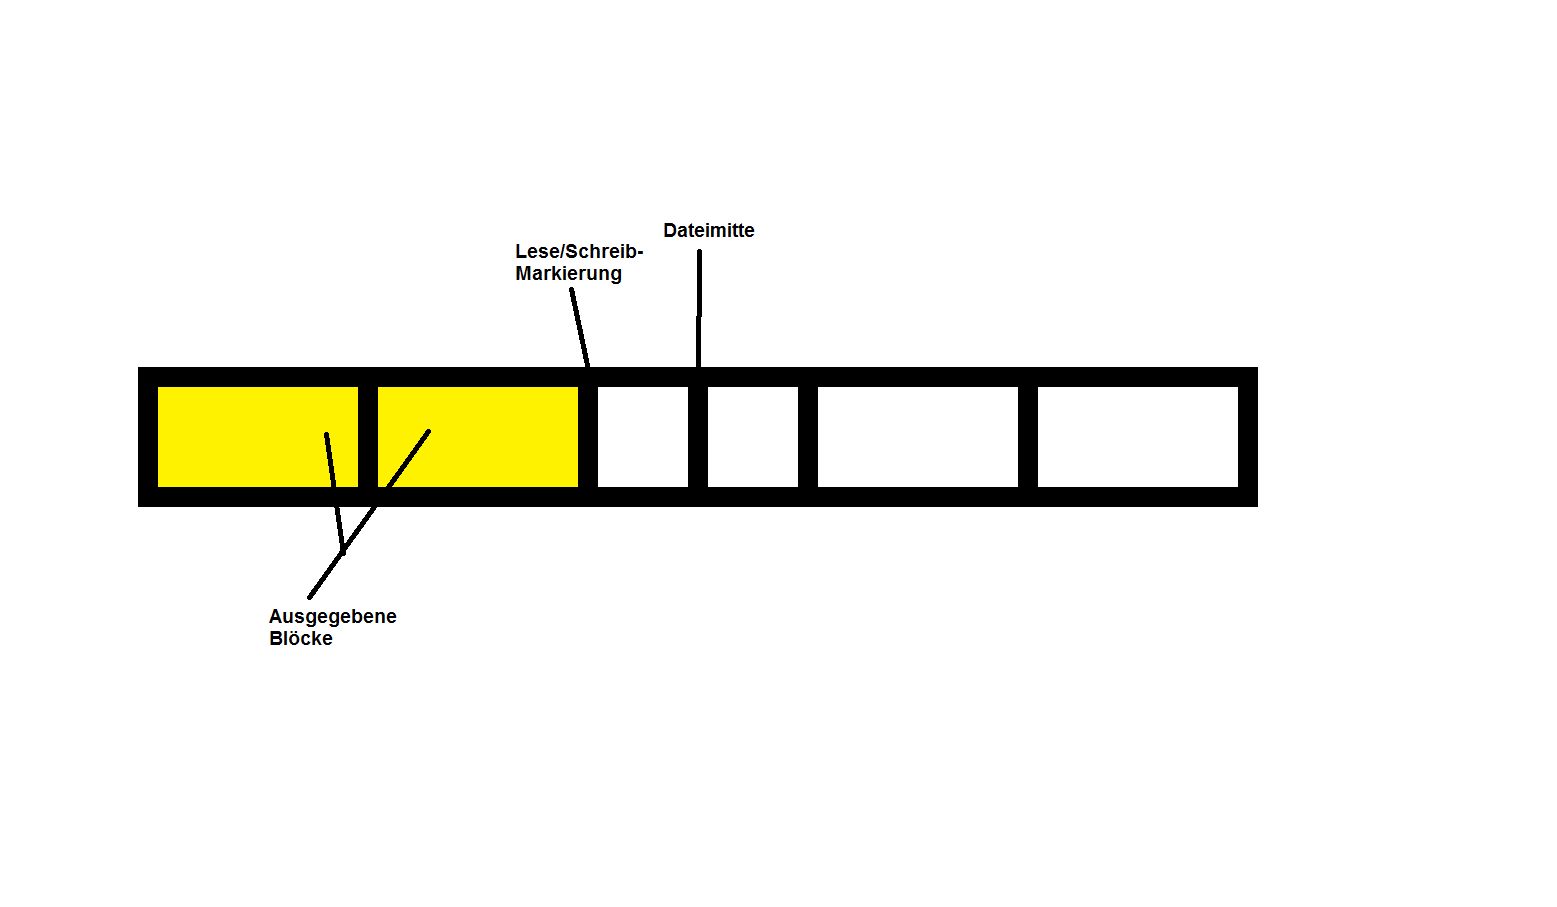
\includegraphics[width=0.7\linewidth]{content/Bsp1}\\
			Dann wird die Anzahl der restlichen Daten mit ''count = dateiMitte \% MAXBYTES;'' berechnet und dann mit ''write()'' ausgegeben. Dabei steht die Eins f\"ur ''stdout''.\\ \\
			
			Aufgabe 8..1.2-4 + Hinweis 4:\\ \\
			\small\lstinputlisting[language=C, firstline=19, lastline=49]{../src/mycp.c}
			\normalsize Erlaubte Programmaufrufe:\\
			\begin{itemize}
				\item ./mycp <Quelldatei> <Zieldatei>\\
				\item ./mycp -o <Quelldatei>\\
				\item ./mycp -o <Quelldatei> <Zieldatei>\\
				\item ./mycp <Text> <Quelldatei> <Zieldatei> (<Text> wird nicht beachtet)\\
			\end{itemize}
			Der Flag ''-o'' legt fest das die Datei auf ''stdout'' ausgegeben wird. Die Quelldatei und die Zieldatei d\"urfen nicht gleich sein. ''argc'' muss mindenstens gleich Drei sein. Wenn ''argc'' gleich Drei ist dann wird mit der Funktion ''isStdout()'' gepr\"uft ob bei ''argv[1]'' der ''o-Flag'' gesetzt ist wenn ja dann ist die Quelldatei in ''argv[2]'' ansonsten ist die Quelldatei in ''argv[1]'' und die Zieldatei in ''argv[2]''. Wenn ''argc'' gleich Vier ist dann ist die Quelldatei in ''argv[2]'' und die Zieldatei in ''argv[3]''. Auch hier wird mit der Funktion ''isStdout()'' gepr\"uft ob bei ''argv[1]'' der ''o-Flag'' gesetzt ist. Danach wird mit ''strCompare()'' verglichen ob Quelldatei und Zieldatei gleich sind. Zuletzt werden die drei Parameter der Funktion ''mycp()'' \"ubergeben.\\ \\
			isStdout():\\ \\
			\small\lstinputlisting[language=C, firstline=51, lastline=70]{../src/mycp.c}
			\normalsize	Die Funktion ermittelt ob der \"ubergebene String gleich ''-o\textbackslash 0'' ist wenn ja dann ist der r\"uckgabe Wert Eins ansonsten Null.\\
			Dabei wird jeden Zeichen eine Gewichtung zugeordnet:\\
			\begin{itemize}
				\item 0 - ''\textbackslash 0''\\
				\item 1 - Jedes Zeichen außer ''-'' und ''o'\\ 
				\item 2 - ''-''\\
				\item 3 - ''o''\\
			\end{itemize}
			Die Gewichte der einzelnen Zeichen werden dann zusammen gerechnet wobei vorher das Gewicht mit einen Faktor multipliziert wird. Der Faktor ist abh\"angig von der Position:\\
			\begin{itemize}
				\item 1 Stelle: Faktor =   1\\
				\item 2 Stelle: Faktor =  10\\
				\item 3 Stelle: Faktor = 100\\
			\end{itemize}
			F\"ur ''-o\textbackslash 0'' ergibt das 32.\\ \\
			strCompare():\\ \\
			\small\lstinputlisting[language=C, firstline=72, lastline=86]{../src/mycp.c}
			\normalsize Die Funktion strCompare() vergleicht ob die Zwei \"ubergebenen Strings gleich sind. Wenn ja dann wird Eins zur\"uck gegeben ansonsten Null.\\
			Dabei werden die Strings zeichenweise verglichen. Wenn die Zeichen nicht gleich sind wird Null zur\"uck gegeben.\\ \\
			mycp():\\ \\
			Die Funktion mycp f\"urt die Dateioperationen aus. Der Parameter ''isstdout'' steht f\"ur den ''o-Flag''. Die anderen Zwei Parameter sind die Quelldatei und die Zieldatei. Bei Erfolg wird Null zur\"uck gegeben ansonsten Eins.\\
			F\"ur denn ersten Teil der Funktion siehe Aufgabe 8.1.1.\\
			\small\lstinputlisting[language=C, firstline=121, lastline=145]{../src/mycp.c}
			\normalsize Wenn der ''o-Flag'' gesetzt ist wird die Variable ''dateineu'' gleich Eins gesetzt. Ansonsten wird die Zieldatei mit ''open()'' ge\"offnet.\\
			\begin{itemize}
				\item O\_WRONLY - die Datei wird nur zum Schreiben ge\"offnet.\\
				\item O\_CREAT - falls die Datei nicht vorhanden ist wird sie erstellt.\\
				\item O\_TRUNC - der Inhalt der Datei wird gel\"oscht.\\
				\item S\_IRWXU - setzt die rwx-Rechte f\"ur den Eigent\"umer.\\
				\item S\_IRWXG - setzt die rwx-Rechte f\"ur die Gruppe.\\
			\end{itemize}
			Danach wird mit ''lseek()'' die Lese/Schreib-Makierung zum Anfang verschoben. Dann wird mit ''read()'' die Datei blockweise gelesen und dann mit ''write(dateineu, buffer, count);'' in die neue Datei bzw. ''stdout'' geschrieben. Das wird solange wiederholt bis das Dateiende erreicht ist. Dann wird mit ''lseek(datei, -11L, SEEK\_END);'' die Lese/Schreib-Markierung zum Zehnt-Letzten Zeichen verschoben. Die Zehn Zeichen werden noch mal eingelesen und dann mit ''write()'' in die neue Datei geschrieben. Am ende werden beide Dateien geschlossen.\\ \\
			Hinweis 1-3:\\ \\
			Verwendet wurden die Funktionen open(), lseek(), read(), write() und close().\\ \\
			Hinweis 5:\\ \\
			Durch das blockweise lesen bzw. schreiben ist das Programm nicht von der Datei-Gr\"oße abh\"angig.\\ \\
			Hinweis 6:\\ \\
			Die Fehlerausgabe wird zuerst in ein char-Array gespeichert und dann mit ''write(2, \&output, sizeof(output));'' aus gegeben. Die Zwei steht f\"ur ''stderr''.\\ \\
			Hinweis 7/Quellen:\\ \\
			\begin{itemize}
				\item http://pubs.opengroup.org/onlinepubs/009695399/functions/read.html Aufruf: 14.06.2016\\
				\item http://pubs.opengroup.org/onlinepubs/009695399/functions/lseek.html Aufruf: 14.06.2016\\
				\item http://pubs.opengroup.org/onlinepubs/009695399/functions/write.html Aufruf: 14.06.2016\\
				\item http://pubs.opengroup.org/onlinepubs/009695399/functions/open.html Aufruf: 14.06.2016\\
				\item http://openbook.rheinwerk-verlag.de/c\_von\_a\_bis\_z/\\016\_c\_ein\_ausgabe\_funktionen\_026.htm Aufruf: 14.06.2016\\
			\end{itemize}
		\end{quote}